\documentclass[12pt]{book}

\usepackage{suthesis-2e}
\usepackage{url}
\usepackage{graphicx}
\usepackage{caption}
\usepackage{subcaption}
\usepackage[inline]{enumitem}
\usepackage{eso-pic}

\counterwithout{figure}{chapter}
\counterwithout{table}{chapter}


\begin{document}

    \title{Comparing Conditional Random Fields and LSTM Networks for Named Entity Recognition}
    \author{Josef Gugglberger}
    \principaladviser{Dipl.-Ing.Clemens Sauerwein, PhD}
	\AddToShipoutPicture*{
		\put(-55,55){
			\parbox[b]{\paperwidth}{
				\hfill \includegraphics[scale=0.35]{img/uni-watermark}
			}
		}
	}
    \beforepreface
    \prefacesection{Abstract} 
    
    In this report, two named entity recognition systems are presented. While one system was implemented with a traditional machine learning approach (Conditional Random Fields), the second system was realised with a deep learning approach (Long-Short-Term-Memory networks). The systems were evaluated on two different datasets: the CoNLL 2003 and the W-NUT 2017 dataset. It was shown that the deep learning approach outperforms the machine learning approach on the CoNLL 2003 dataset. However, on the noisy W-NUT 2017 dataset, the machine learning approach performed better.

 	\afterpreface
 	
 	
    \chapter{Introduction}
    
    With the rise of deep learning from 2015 onwards, the methods to perform named entity recognition (NER) have changed in research. The traditional machine learning approaches like Hidden Markov Models and Conditional Random Fields (CRF) were mostly replaced by a special type of Recurrent Neural Networks, so-called Long-Short-Term-Memory networks (LSTM). The first approach to apply LSTM networks for named entity recognition was done already in the year 2003 in the paper \cite{hammerton-2003-named}. However, due to the lack of computational power back then, the performance was far behind state-of-the-art methods. In 2015, Huang et al. \cite{huang2015bidirectional} showed various LSTM networks that reached state-of-the-art performance. Also, the currently best performing NER system on the CoNLL 2003 \cite{sang2003introduction} dataset, called \textit{Flair} \cite{akbik2018contextual}, makes use of a LSTM network. \\
    
    Aim of this work is to perform a practical study, comparing the performance of a machine learning approach, and a deep learning approach on two well-studied datasets. The study was conducted by implementing two NER systems: the first system is based on CRFs, while the second system implements two variations of a bidirectional LSTM (BI-LSTM) network. The performance of the tools are compared in terms of precision, recall and F1-score on the CoNLL 2003 and the W-NUT 2017 \cite{derczynski2017results} dataset. \\
    
    The remainder of this thesis is structured as follows: Chapter \ref{chap:backround} is about related work and some background information on named entity recognition, CRFs and LSTM networks. Next, Chapter \ref{chap:method} describes the details of the two implementations of the NER system. Chapter \ref{chap:evaluation} compares the results generated by the previous chapter. Finally, Chapter \ref{chap:conclusion} concludes and give an outlook on what can be done in future works.
   
	\chapter{Background \& Related Work}
	\label{chap:backround}
	
	This chapter presents basic background information of the topics NER (Section \ref{sec:ner}), CRFs (Section \ref{sec:crf}) and LSTM networks (Section \ref{sec:lstm}). The last section, Section \ref{sec:relatedwork}, summarizes the recent work that was done in comparisons between CRFs and LSTM networks.

	
	\section{Named Entity Recognition}
	\label{sec:ner}
	
	\textit{Named entity recognition} is the task of locating and classifying named entities in unstructured text. A named entity is classified into a predefined set of categories, which can be names of people, locations, companies, etc. A named entity describes something physical (person, location, etc.), and a \textit{mention} is a phrase in the text that refers to that entity with a name \cite{MAL-013}. For example, the terms \textit{U.S.A} and \textit{the United States of America} are two different phrases that refer to the same named entity.
	
	The categories in which the named entities are classified depends strongly on the domain where the NER system will be deployed, but the categories \textit{person}, \textit{location}, \textit{organization} and \textit{miscellaneous} are often used in research, for example in \cite{tjongkimsang2003conll}.
	 
	According to AclWeb \cite{conll-sota}, the current state of the art approach on the CoNLL-2003 dataset reaches an F1 score of 93.09 \%.
	
	\section{Conditional Random Fields}
	\label{sec:crf}
	
	A \textit{Conditional Random Field}, initially proposed in \cite{lafferty2001conditional}, is a discriminative probabilistic classifier. In contrast to a discrete classifier (like the naive Bayes classifier), it makes its prediction not just based on the input sample, but also based on the context of the input sample. This is an important feature in the domain of natural language processing, especially in part-of-speech tagging and named entity recognition. 
	
	To model the context of a sample we have to define feature functions, which have to be defined in a way that expresses some characteristic that is present in the training data and that is expected to be present in the test data. A feature function has to form:
	
	\begin{equation}
	f(y_t, y_{t-1}, x_t)
	\end{equation}
	
	where $y_t$ is the current label, $y_{t-1}$ is the previous label and $x_t$ are the samples from the input sequence that the feature function needs to calculate the feature. The Conditional Random Field, as defined in \cite{MAL-013}, is then:
	
	\begin{equation}
	p(y|x) = \frac{1}{Z(x)} \prod_{t=1}^T exp(\sum_{k=1}^{K} \theta_k f_k(y_t, y_{t-1}, x_t))
	\end{equation}
	
	where $Z(x)$ is an normalization function:
	
	\begin{equation}
	Z(x) = \sum_{y} \prod_{t=1}^{T} exp(\sum_{k=1}^{K} \theta_k f_k(y_t, y_{t-1}, x_t))
	\end{equation}
	
	and $\theta$ is a parameter vector. The values of the parameter vector $\theta$ have to be learned from the training data, usually via Maximum Likelihood Estimation. Each feature function is multiplied by its parameter vector and then summed up. To take the context into account, this is computed for every time-step, which are then multiplied by each other. The result is $p(y|x)$, which is the probability of $y$ (the named entity label) over $x$ (the word). This probability is calculated for each named entity category, and the maximum is chosen as the prediction.
	
	\section{LSTM Networks}
	\label{sec:lstm}
	
	A LSTM network is a special type of Recurrent Neural Network (RNN). In contrast to a feed-forward neural network, like for example a Convolutional Neural Network, where the data flows only in one direction (from input to output), the data can flow in cycles in a RNN. This property makes a RNN able to memorize inputs, which causes them to be suitable for sequence labelling tasks.
	RNNs have been considered difficult to train a long time, especially when they are trained to recognise long-term dependencies. The problems that arise in such cases is called the \textit{vanishing} and \textit{exploding} gradient problem \cite{lipton2015critical}. The vanishing gradient problem occurs because the gradients of back-propagation are multiplied by each other to get the dependencies from the previous steps. This problem makes RNNs almost unusable for many NLP tasks because natural language can rely heavily on long-term dependencies.
	
	LSTM networks, proposed in \cite{hochreiter1997long}, were designed to overcome the issue that RNNs have with long-term dependencies. Each LSTM cell holds an internal memory state, which is added (instead of multiplied) to the process input. The time dependence in the cell is determined by the forget gate.
	
	Figure \ref{img:lstm} shows a LSTM cell. The data flows from left to right. $x$ is the sequence sample at the current time step, $o-1$ is the output of the previous LSTM cell. The input $x$ and $o-1$ are concatenated at the first step and is squashed between -1 and 1 by a $tanh$ function afterwards. The result of this is then multiplied element-wise with the output of the input gate. The \textit{input} gate is a sigmoid function, mapping inputs between 0 and 1, this can turn on and off parts of the input. 
	The next stage in the cell is called the \textit{forget} gate. The new variable $s$ represents the internal state of the LSTM cell. The internal state is delayed by one step (represented by $s-1$) and added to the output of the input gate. A sigmoid function determines which words can be forgotten (close to 0), and which words need to be remembered (output close to 1).
	The last stage is the \textit{output} gate, which operates in the same way as the input gate. The output is squashed between -1 and 1 by a hyperbolic tangent function and the output gate with a sigmoid function determines which values to output.
	
	\begin{figure}
		\begin{center}
			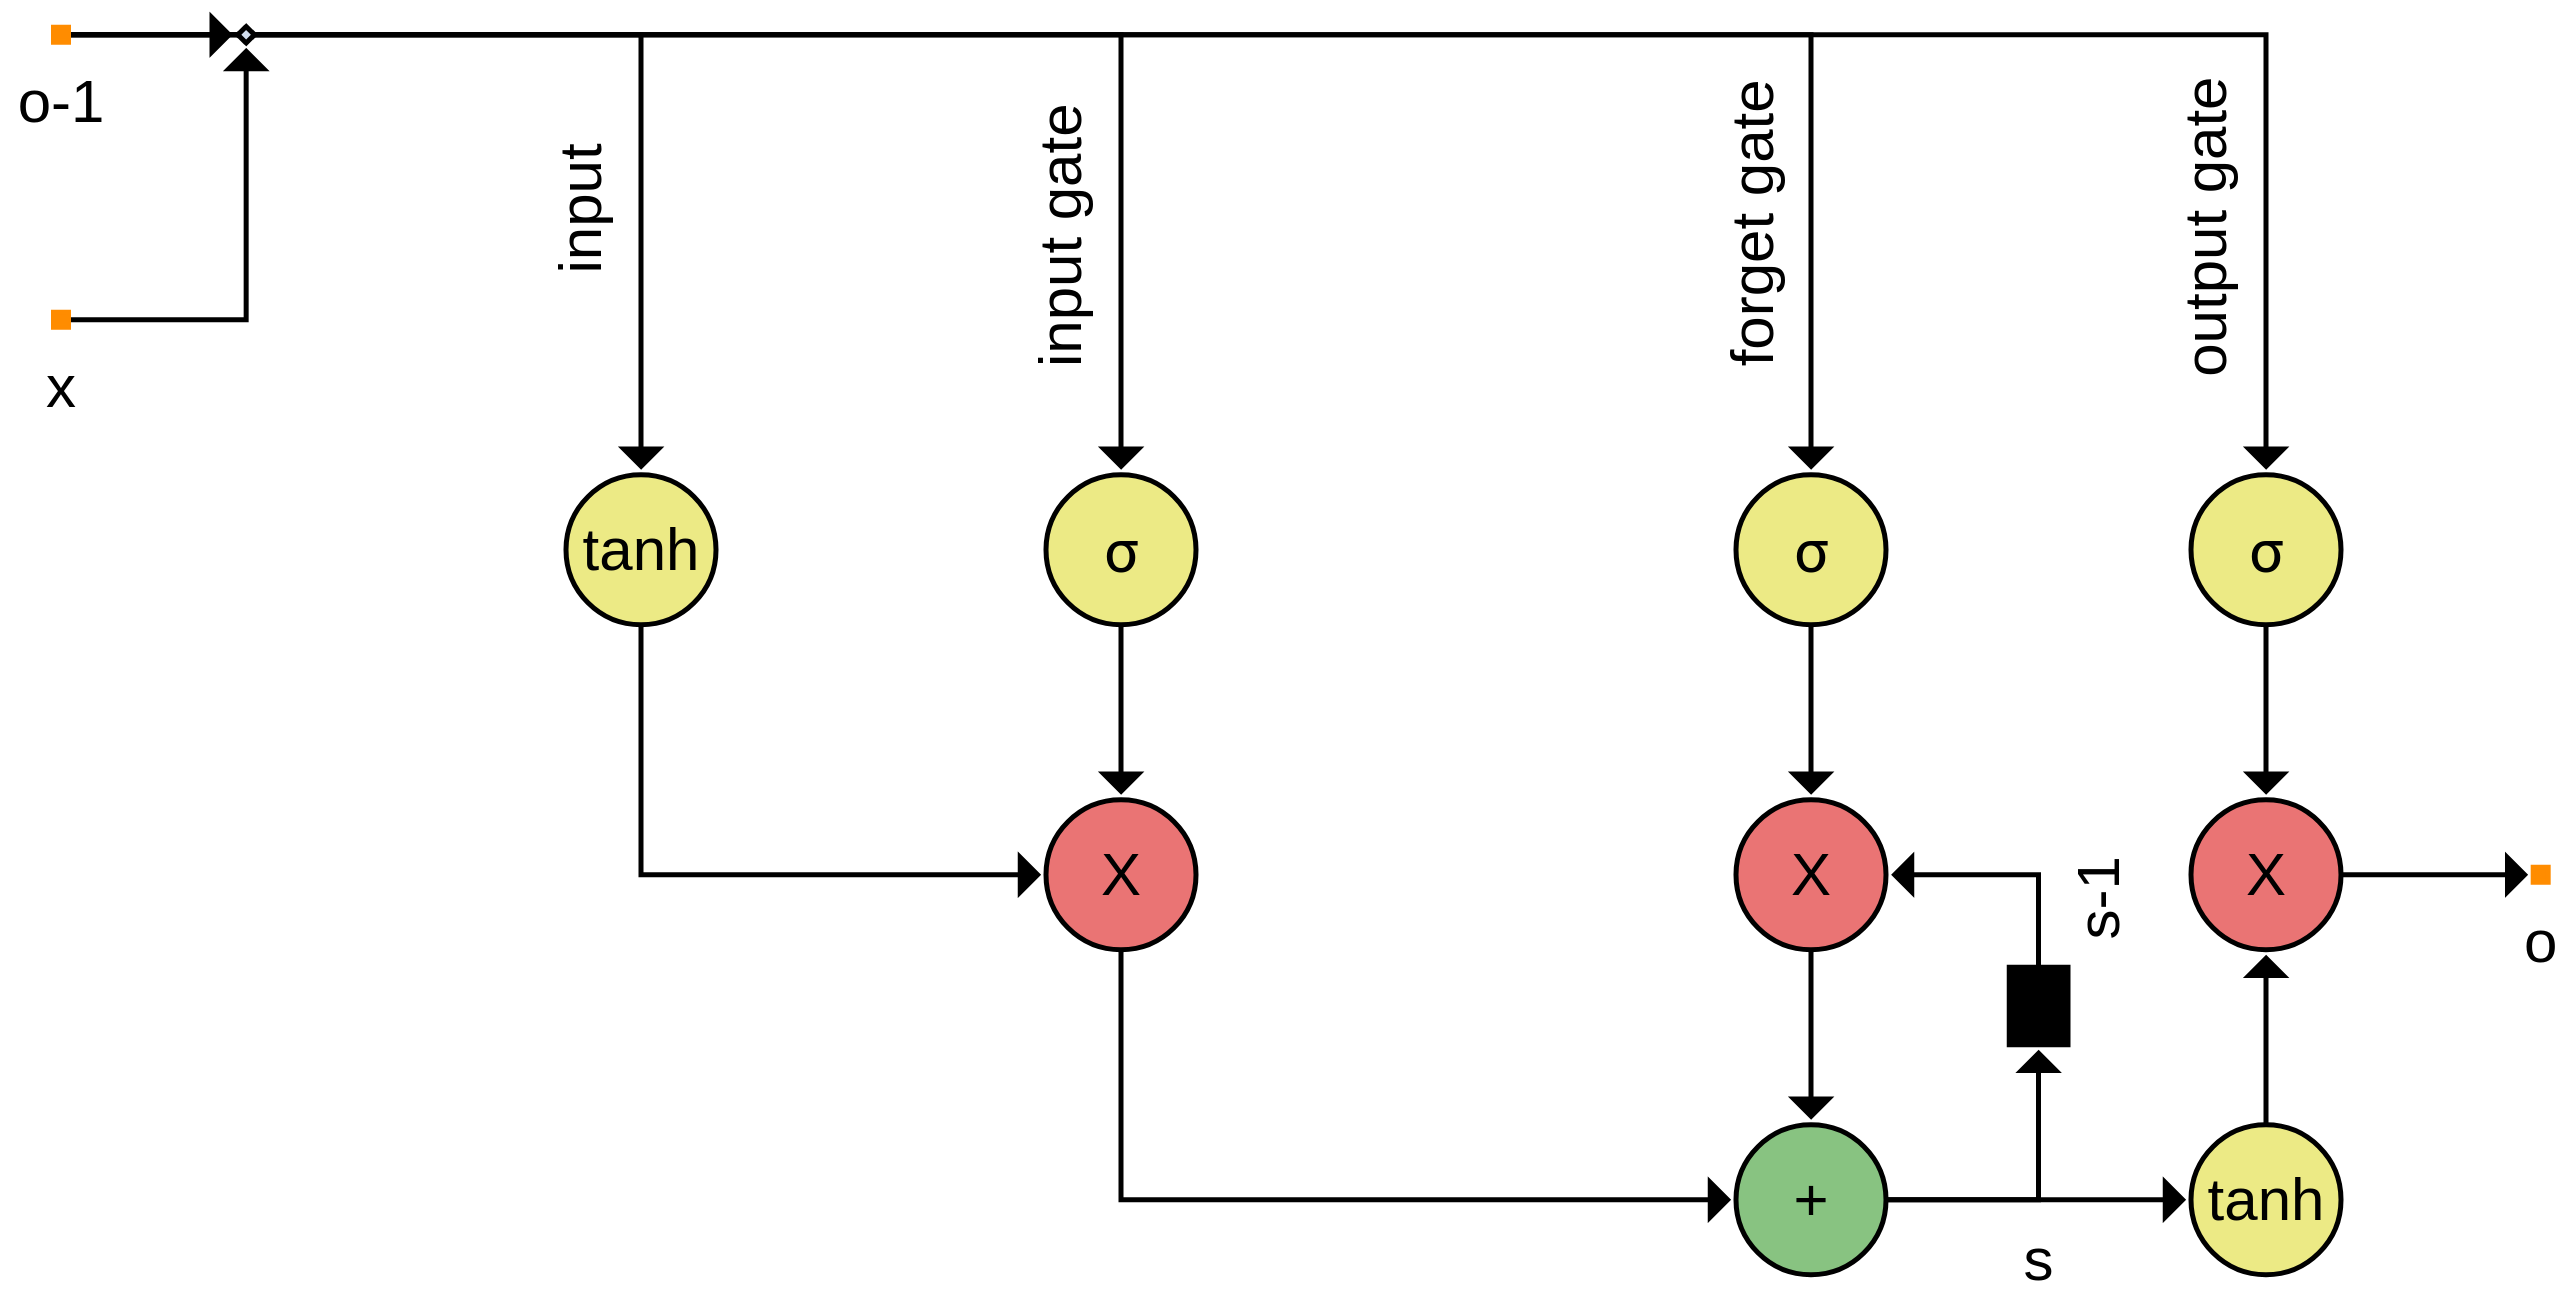
\includegraphics[width=0.75\linewidth]{img/lstm.png}
		\end{center}
		\caption{Overview of a LSTM cell. Yellow nodes represent a hidden layer, red and green nodes represent a element-wise operation.}	
		\label{img:lstm}
	\end{figure}
	
	\section{Related Work}
	\label{sec:relatedwork}
	
	A comparison between CRF and LSTM networks was already proposed by Nikola Ljube{\v{s}}i{\'c} in \cite{ljubevsic2018comparing}. However, there are some differences in the scope of the study: first, the analysis that was made there focuses on Slovene, Croatian and Serbian data, second, the paper concentrated on morphosyntactic tagging instead of NER, and third, the study was just based on short and noisy posts from Twitter. The author concluded that both approaches performed with good and also similar results. He conducted a error-analysis, which showed that the neural network worked better at long-range dependencies, while CRFs performed slightly better at local dependencies. Furthermore, the author claims that the neural network performed better in comparison to the CRF system with increasing \textit{non-standardness} of the text.
	
	\chapter{Method}
	\label{chap:method}
	
	Aim of this work was to conduct a practical study comparing a CRF approach and a LSTM approach for NER. Two NER systems were developed, trained and tested by two different datasets. This chapter provides the implementation details of both approaches.
	
	\section{Dataset}
	
	Two very different datasets were used to train and test the NER systems. On the one hand, the famous CoNLL 2003 \cite{sang2003introduction} dataset, which consists of newswire articles from the Reuters corpus, and on the other hand the W-NUT 2017 \cite{derczynski2017results} dataset, which consists of noisy user-generated text, were used.
	
	\section{Implementation}
	
	The following section presents the implementation details of the developed NER systems. Subsection \ref{sub:CRF} starts with presenting the CRF approach. Second, Subsection \ref{sub:lstm} continues with the details of the LSTM approaches.
	
	\subsection{Conditional Random Fields}
	\label{sub:CRF}
	
	The CRF approach was implemented with the help of the following Python libraries: \textit{python-crfsuit} \cite{pycrfsuite}, \textit{nltk} \cite{nltk} and \textit{gensim} \cite{gensim}.
	
	A lot of effort was invested to come up with a good working feature set. The employed feature functions can be grouped into five categories: \begin{enumerate*}
		\item word-based features,
		\item sentence \& collection-based features,
		\item dictionary-based features, 
		\item features form other NLP tasks, and
		\item features from unsupervised machine learning algorithms.
	\end{enumerate*}

	\subsubsection{Word-based features}
	
	Following characteristics were defined as word-based features:
	\begin{itemize}
		\item length of word
		\item word starts with an upper-case letter
		\item word contains an upper-case letter
		\item word contains a digit
		\item word contains a special character
		\item shape of the word ('Word' maps to 'Aa+', 'WORD' maps to 'A+', 2020-01-16 maps to 9999\#99\#99)
	\end{itemize}
	
	\subsubsection{Sentence \& collection-based features}
	
	Following characteristics were defined as sentence and collection-based features:
	\begin{itemize}
		\item position of word in sentence
		\item number of occurrences in collection
	\end{itemize}
	
	\subsubsection{Dictionary-based features}
	
	For gathering dictionary features each word was looked up in multiple dictionaries. Following dictionaries where used:
	\begin{itemize}
		\item stop-words list by nltk corpus
		\item name-list by nltk corpus
		\item word-list by nltk corpus
		\item Length of hypernym path in WordNet \cite{wordnet}. This gives some kind of information like the specificness or rareness of a word.
	\end{itemize}

	\subsubsection{Features from other NLP tasks}
	
	The part-of-speech (POS) tag, which was extracted by the help of the library \textit{nltk}, was used as a feature.
	
	\subsubsection{Features from unsupervised machine learning algorithms}
	Several features were collected from unsupervised ML clustering algorithms. The cluster which the word appears in is used as a feature value.
	Following algorithms were used:
	\begin{itemize}
		\item Brown cluster \cite{brown1992class}. The cluster where the word is in and the bit-sequence returned from the algorithm is used as a feature. The best results were achieved with five clusters.
		\item Latent Dirichlet Allocation (LDA) \cite{blei2003latent}. LDA is used to model the abstract topic of a document. It returns a distribution of topics per word. The most dominant topic of each word was used as a feature. The best results were achieved with three topics.
		\item Word2Vec cluster \cite{w2vgensim}. Word2Vec learns relationships between words, and outputs one vector for each word. It maps similar words to similar vectors. The vector is used as a feature.
	\end{itemize}
	
	\subsection{LSTM Network}
	\label{sub:lstm}
	
	For the implementation of the two variants of LSTM networks the Python deep learning package Keras \cite{keras} was used with TensorFlow \cite{tensorflow} as a back-end. The two implemented approaches were first proposed by Huang et al. in \cite{huang2015bidirectional}. Both proposals use a bidirectional LSTM layer, which means that the LSTM network is duplicated. The input as-is is feed into the first layer, the input reversed is feed into the second layer. This can be beneficial because it requires contextual information about past (words to the left of current) and future (words on the right of current) words to correctly classify a named entity.
	
	The Keras model of the BI-LSTM approach is shown in figure \ref{fig:lstm}. After the input layer, strings are converted to vectors in the embedding layer. The embedding layer was pre-trained with GloVe \cite{glove} embeddings with a vector size of 100. After embedding the words, a Dropout layer is applied to avoid over-fitting. The theory behind the Dropout layer was proposed by Srivastava et al. in \cite{srivastava2014dropout}. The key idea is to randomly drop a defined amount of units in training. The dropout rate was set to $0.2$ in the tool. Next, the data flows into the bidirectional LSTM layer. A time distributed dense layer is then applied before output. A time distributed dense layer is used here instead of a normal dense layer because of the sequential nature of natural language: there is one output (named entity label) per time-step or word.

	\begin{figure}
		\begin{center}
			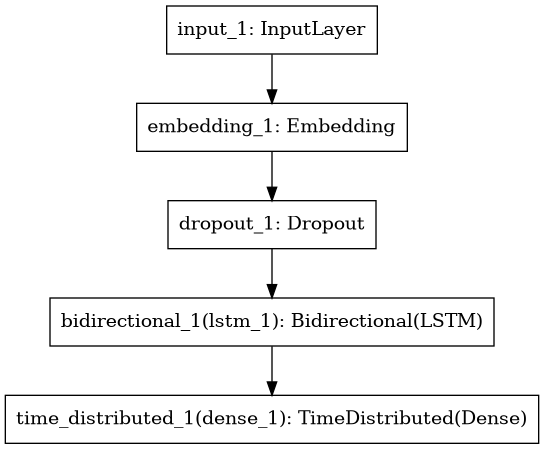
\includegraphics[width=0.4\linewidth]{img/lstm_model.png}
		\end{center}
		\caption{Keras model of NER system with Bidirectional-LSTM network.}
		\label{fig:lstm}
	\end{figure}

	The Keras model of the BI-LSTM-CRF approach is shown in figure \ref{fig:lstm}. It is the same model as described in the previous paragraph, with an additional CRF layer added at the bottom. It is a combination of the first presented CRF approach and the BI-LSTM approach presented before. The CRF layer has the advantage that it does also capture sentence level tag information, instead of just using past and future features as the BI-LSTM approach.
	
	\begin{figure}
		\begin{center}
			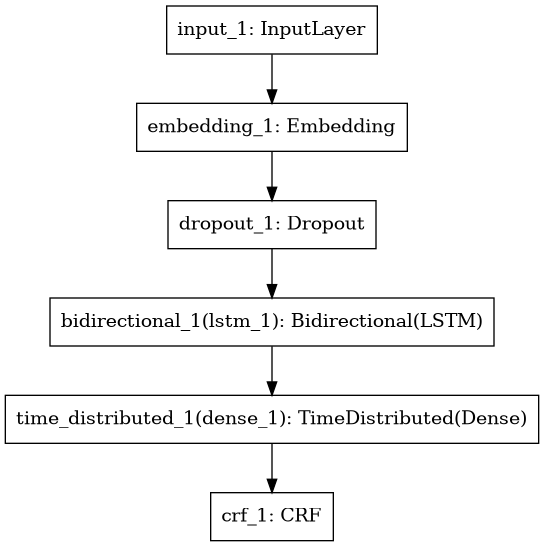
\includegraphics[width=0.4\linewidth]{img/lstm_crf_model.png}
		\end{center}
		\caption{Keras model of NER system with Bidirectional-LSTM-CRF network.}
		\label{fig:lstm-crf}
	\end{figure}
	

	\chapter{Evaluation \& Comparison}
	\label{chap:evaluation}
	
	Table \ref{tab:res_conll} and \ref{tab:res_wnut} display the results of the various implemented NER systems, together with a state-of-the-art approach called \textit{Flair} \cite{akbik2019flair}. The evaluation was done, as described in \cite{tjongkimsang2003conll}, by marking predicted named entities as correct \textit{iff} it is an \textit{exact} match with the test data file. The implemented approaches where trained with a train test split of 85\% / 15\%, the results are therefore not completely comparable with other participants of the CoNLL and W-NUT competition.
	
	Table \ref{tab:res_conll} shows precision, recall and F1-score on the CoNLL 2003 dataset. The general observing of this table is that the deep learning approaches BI-LSTM and BI-LSTM-CRF performed better than the machine learning approach CRF on all metrics.
	
	Table \ref{tab:res_wnut} show precision, recall and F1-score on the W-NUT 2017 dataset. The key finding here is that the CRF and BI-LSTM-CRF approaches performed much better than the non-CRF approach BI-LSTM.
	
	Both tables also show the state-of-the-art approach called \textit{Flair}. Flair also uses a BI-LSTM-CRF model, but it was implemented with the deep learning library PyTorch \cite{pytorch} instead of Keras. What makes their approach different is a new type of string embedding, proposed by Akbik et al. in \cite{akbik2018contextual}.
	
	\begin{table}
		\begin{center}
			\begin{tabular}{| l | c | c | c |}
				\hline
				Method & Precision & Recall & F1-score \\ \hline
				CRF & 84.25 & 85.42 & 84.83 \\ \hline
				BI-LSTM & 84.37 & \textbf{86.58} & 85.46 \\ \hline
				BI-LSTM-CRF & \textbf{89.41} & 86.20 & \textbf{87.78} \\ \hline
				Flair & - & - & 93.09 \\ \hline
			\end{tabular}
		\end{center}
		\caption{Results on CoNLL 2003 dataset.}
		\label{tab:res_conll}
	\end{table}
	\begin{table}
		\begin{center}
			\begin{tabular}{| l | c | c | c |}
				\hline
				Method & Precision & Recall & F1-score \\ \hline
				CRF & 31.54 & \textbf{56.72} & \textbf{40.53} \\ \hline
				BI-LSTM & 8.69 & 23.16 & 12.63 \\ \hline
				BI-LSTM-CRF & \textbf{33.61} & 31.03 & 32.27 \\ \hline
				Flair & - & - & 49.49 \\ \hline
			\end{tabular}
		\end{center}
		\caption{Results on W-NUT 17 dataset.}
		\label{tab:res_wnut}
	\end{table}

	\chapter{Conclusion}
	\label{chap:conclusion}
	
	The results shown in chapter \ref{chap:evaluation} didn't show a clear picture of which approach should be favoured. Although the LSTM approach worked better on the CoNLL 2003 dataset, CRF performed very well on the noisy W-NUT 2017 dataset.
	A comparison between the proposals in terms of working hours that it took to set up the NER systems as they are, can be made. Because of the large amount of feature engineering that has to be done for the CRF approach, it took longer to implement that approach in comparison to the LSTM approach. But not just the implementation was more work, also the fine-tuning and feature selection is more time-intense because there are much more parameters that have to be determined in a trial and error fashion.
	The developed BI-LSTM(-CRF) based systems have more potential for further improvement. Different string embeddings could be used. Instead of training embeddings from scratch or using pre-trained embeddings like GloVe, using more recent embedding techniques, like BERT \cite{devlin2018bert}, ELMo \cite{peters2018deep} or Flair \cite{akbik2018contextual} embeddings would enhance the performance of the tool. 
	BI-LSTM-CRF is the current state-of-the-art method to many NLP tasks, including NER. Unless the data isn't very noisy it should be preferred over a CRF approach.
	
	\bibliographystyle{plain}
	\bibliography{thesis}

\end{document}
